\documentclass[12pt, a4paper]{scrartcl}
\usepackage[german]{babel}
\usepackage[utf8]{inputenc}
\usepackage{graphicx}

\begin{document}
\section{Funktionsumfang und Eingabeverarbeitung auf der Anwendungsebene}

\subsection{Entwicklung einer eigenen Scriptsprache zur Anwendungssteuerung}
\subsubsection{Theoretische Grundlagen formaler Sprachen}
Wir als Menschen haben die gesprochenen Sprachen entwickelt, um uns untereinander zu verständigen und Informationen auszutauschen. Um Misverständnisse zu vermeiden, folgt unsere Kommunikation strikten Grammatikalischen und Semantischen Regeln. Es werden strukturelle Merkmale wie zum Beispiel die Reihenfolge einzelner Sprachteile festgelegt. Außerdem gibt es einen begrenzten Wortschatz, indem Jedes Wort eine bestimmte Bedeutung hat.  
\subsubsection{Spezifikation unserer Scriptsprache anhand unserer Ansprüche an den Funktionsumfang}

\subsection{Implementierung der Anwendungssteuerung in der Scriptsprache Lua}

\subsubsection{Darstellung des grundlegenden Programmaufbaus und Programmablaufs}
Grundlegende Aufgabe der Anwendungssteuerung ist es, die Eingaben die der Nutzer unserer Software tätigt, in Aktionen des Programms umzusetzten. Dazu werden zum einen auf dem Rechner der sendenden Person die, nach der in Kaptiel x.1 beschriebenen Syntax, eingegebene Anweisung in der Eingabeverarbeitung auf ihre Korrektheit überprüft, um anschließend aufgeschlüsselt zu werden und die gewünschte Sendefunktion zu initialisieren.\\
Nachdem die Daten mithilfe des Netzwerkprotokolls übermittelt wurden, werden sie von der Übertragungsverarbeitung, auf dem Empfängercomputer weiter bearbeitet. Je nach spezifiziertem Typ der Übermittlung, wird entweder die enthaltene Datei auf Fehler überprüft und anschließend endgültig gespeichert, oder die auszuführende Anweisung wird an die betirebsystemeigene Kommandozeile weitergegeben und ausgeführt.\\
Um keine ungewollten Übertragungen von potenziell schädlichen Dateien oder Anweisungen zu ermöglichen, wird für die Ausführung jeder Übermittlungsanfrage die Bestätigung des Empfängers benötigt.\\\hfill\\
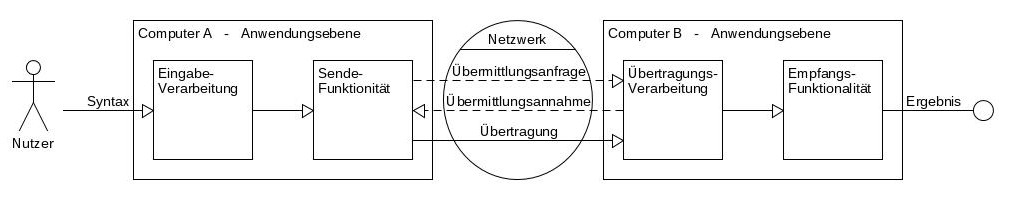
\includegraphics[scale=.45]{anw.jpg}
\subsubsection{Ansprüche an die Implementierung und die daraus resultierende Wahl der Programmiersprache}
Wie in Kapitel 3.2.1 erläutert, wird auf der Anwendungsebene unseres Programmes, also dem Teil welcher ausschließlich auf einem Rechner läuft, die grundlegende Funktionalität implementiert. Da unser selbstentwickeltes Netztwerkprotokoll, welches die eigendliche Kommunikation zwischen 2 Computern bewirkt, relativ universell auf verschiedenartige Daten anwendbar ist, stellt dieses im Bezug auf den Funktionsumfang der Software nicht den limitierenden Faktor da. Um das Protokoll eventuell auch im Zeitraum nach der eigendlichen Arbeit ausnutzen zu können, und nicht durch einen festgelegten Satz von Befehlen beschränkt zu werden, entschieden wir uns dazu, diese Softwareebene in einer Scriptsprache zu implementieren.\\
Diese Klasse von Programmiersprachen kennzeichnet sich dadurch aus, dass der vom Menschen lesbare Quelltext eines Programmes erst bei seiner Ausführung in Anweisungen übersetzt werden, welche für den Computer ausführbar sind. Im gegensatzt zu kompilierten Sprachen hat dies den Vorteil, dass Programmcode unkompliziert korrigiert und modifiziert werden kann.\\
In diesem Zusammenhang ergibt sich außerdem eine leichte Wartbarkeit, also die Möglichkeit eventuell auftretende Fehler zu beseitigen, als ein weiterer erfüllter Anspruch. Da wir stets zu dritt an unserer Software programmiert haben, sollte es jedem von uns mit möglichst geringem Aufwand möglich sein, Programmteile zu verbessern, auch wenn es sich nicht um den ursprünglichen Autor handelt.\\
Den Vorteil von kompilierten Programmiersprachen, dass sie sich durch eine höhere Leistungsfähigkeit besonders bei komplexeren Problemen auszeichnen, haben wir uns durch die Implementierung unserer Netzwerkteils in der Sprache C++ zu nutzen gemacht. Dies stellt den Anspruch, dass die gewählte Scriptsprache problemlos in Software der Sprache C++ einzubetten ist, und keine Probleme bei der Kommunikation zwischen Programmen der zwei Sprachen auftreten.\\
Da wir als Gruppenmitglieder unterschiedliche Betriebsysteme auf unseren Arbeitsrechnern benutzen, entstand als Nebenprodukt die Anforderung, dass das finale Programm systemunabhängig sein muss, also ohne erheblichen Aufwand auf neue Betriebssysteme portierbar ist. Unser Fokus lag dabei für die Arbeit auf Computersystemen und wir haben mobile Geräte vorerst außen vor gelassen.
Zu guter Letzt ist der Zeitraum der Seminarfacharbeit auch nur auf andertalb Jahre begrenzt, weshalb die gewählte Sprache mit einem geringem Lernaufwand benutzbar sein muss.\\
Als Kompromiss zwischen allen beschriebenen Ansprüchen entschieden wir uns für die Programmiersprache Lua. Da sie in reinem C geschrieben ist, weißt sie eine uneingeschränkte Integrationmöglichkeit unseres Netzwerkprotokolls vor, und lässt sich außerdem auf die meist verbreitesten Betriebssytemarchitekturen wie Windows und Unix portieren.\footnote{www.lua.org/about.html, 17.11.2018} Ein positiver Nebeneffekt dieser Wahl ist die hohe Leistungsfähigkeit von Lua, verglichen zu anderen weit verbreiteten Scriptsprachen. Der Sprachaufbau orientiert sich sehr nah an der Englischen Srache, was ein schnelles Erlernen ermöglichte. 


\subsubsection{Erläuterung wesentlicher Elemente der Implementierung}


\end{document}
